% \vspace*{-.05in}
\section{Program Modules}
\vspace*{-.05in}
There are 8 parts in out program, including \textsl{requirements.txt}, \textsl{model/}, \textsl{preprocess/}, \textsl{static/}, \textsl{utils/}, \textsl{constants.py}, \textsl{data.py} and \textsl{train.py}.

\subsection{requirements.txt}
The content of \textsl{requirements.txt} is the third-party dependencies and their version. This file is generated by the following command.
\begin{lstlisting}[language=bash]
$ pip freeze > requirements
\end{lstlisting}

\subsection{preprocess/}
The module \textsl{preprocess/} is to preprocess the raw data set into fixed formal file. Firstly it reshuffle the data set and then divide the raw data set into train, validation and test set by 80\%, 10\% and 10\%.

As the model optimizes the learnable parameters on the training set, the loss value on the training set is gradually reduced. But when the number iterations is too big, the model will learn the features specific to this training set but not universal features. As a result, the model is overfitting and accuracy decreases.

 So we use training set and validation set to train model and decide whether to early stop. At each iteration, we firstly use training data set to optimize the model with SGD algorithm and respectively calculate average loss values of training data and validation data. If the average loss values of training data or validation data increases 5 times, which means loss value on validation data set has converged and will be overfitting if continue training, we early stop the training.

\subsection{data.py}
\textsl{data.py} is to read the preprocessed data set and store \textsl{train\_source\_data}, \textsl{train\_target\_data}, \textsl{eval\_source\_data}, \textsl{eval\_target\_data}, \textsl{test\_source\_data} and \textsl{test\_eval\_data} in the instance of Class \textsl{Data}. Each instance of target data is an one hot vector full of zero except the position whose index is the relevant category. For example, if the category of a data instance is 2 with 4 categories in all instances, then the target data of this instance is [0, 0, 1, 0].

What's more, the class \textsl{Data} also provide methods to get batch data of train, validation and test sequentially. And there are also some methods to provide the common values such as \textsl{input\_size}, \textsl{output\_size} and \textsl{train\_batches\_sum}.

\subsection{constants.py}
\textsl{constants.py} stores the constant values used in project, including paths static files and suffix of fixed formal data set file. 

\subsection{utils/}
\textsl{utils/} has various tool methods. \textsl{file\_utils.py} is to transform between file and string, transform between JSON file and dict, and make directory if it does not exist. \textsl{log\_utils.py} is to output logs to the console and file. And \textsl{shell\_args.py} is to define the formate of arguments used in shell.

\subsection{model/}
The module \textsl{model/} defines the Neural Network model, with three parts including \textsl{activator/}, \textsl{fully\_connected\_layer.py} and \textsl{neural\_network.py}. 

All calculations in the model use matrix operations by \(numpy\) instead of loops in \(python\). Because matrix operations by \(numpy\) underlying layer is implemented in C++, which is much faster than \(python\).

\subsubsection{Neural Network Model}
\begin{figure}[htbp]
	\centering
	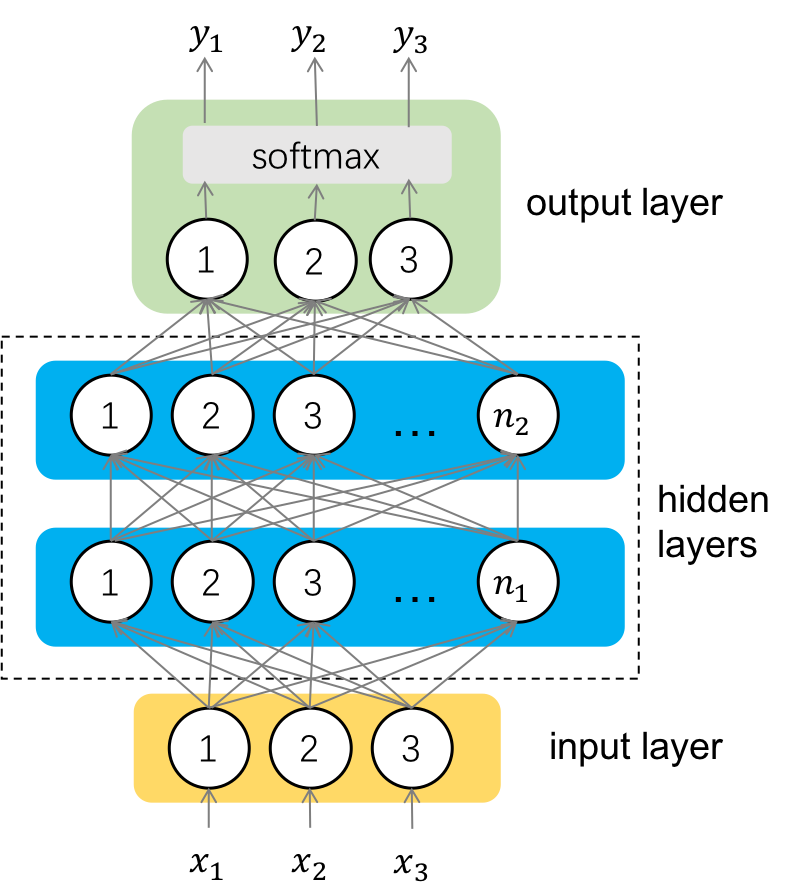
\includegraphics[width = .4\textwidth]{images/dnn.png}
	\caption{The overall structure of full connected Neural Network.}
	\label{fig:dnn}
\end{figure}

We implement the full connected Neural Network shown as Figure \ref{fig:dnn}. Neural networks are actually multiple neurons connected according to certain rules. There are one input layer, output layer, and multiple hidden layers between them.

The number of neurons in input layer is the number of features in source data. The number of neurons in output layer is the number of categories in target data. Each output of neuron in output layer represents the probability of getting this category based on the input features, which is between 0 and 1 and the sum is equal to 1.

For the \(i\)-th layer, the output vector is calculated by the following equation according to the input vector:
% equation for y_{i+1}
\begin{equation}
\boldsymbol{y_{i}} = f(\boldsymbol{x_{i}}\boldsymbol{w_i} + \boldsymbol{b_i})
\end{equation}
where \(\boldsymbol{y_{i}}\) is the output vector, \(\boldsymbol{x_{i}}\) is the input vector, \(\boldsymbol{w_{i}}\) and \(\boldsymbol{b_{i}}\) is the learnable parameters, and \(f\) is the activator function. The activator in output layer is \(softmax\) as follows:
% equation for softmax
\begin{equation}
softmax(z_k) = \frac{e^{z_k}}{\sum_{i=1}^{n}{e^{z_i}}}
\end{equation}
where \(n\) is the output size. Except output layer, the activator in each layer is \(sigmoid\) or \(tanh\) as follows.
% equation for softmax
\begin{equation}
sigmoid(z) = \frac{1}{1 + e^{-z}}
\end{equation}
% equation for tanh
\begin{equation}
tanh(x) = \frac{e^{x} - e^{-x}}{e^{x} + e^{-x}}
\end{equation}

The loss function is the cross entropy calculated by the negative log likelihood:
% equation for sigmoid
\begin{equation}
Loss = \frac{1}{m}\sum_{i=1}^{m}{-t_{i}{\rm log}y_i}
\end{equation}
where \(m\) is the number of categories, \(t_i\) is the target value and \(y_i\) is the predicted value for the category \(i\).

\subsubsection{The Module activator/}
There is a abstract class \(Activator\) with two abstract methods: \(forward\) which is used to calculate output by the input, \(backward\) which is used to calculate the derivative of the activator according to the output calculated by the \(forward\). And the subclass \(SoftmaxActivator\), \(SigmoidActivator\), \(TanhActivator\) respectively implement their respective \(backward\) and \(forward\).

\subsubsection{The Module fully\_connected\_layer.py}
The class \(FullyConnectedLayer\) is represented a layer in Neural Network. It stores and updates the learnable vector \(\boldsymbol{weights}\) and \(\boldsymbol{bia}\). It also provides how to initial the learnable vector such as full of zero, random uniform and random normal.

It provides methods \(forward\) to calculate the output vector according to input, weights, bia and activator, and \(backward\) to calculate the gradient delta according to the gradient of previous layer.
\subsubsection{The Module neural\_network.py}
The class NeuralNetwork define the structure of the model, including the input size, output size, number of hidden layer, the size of each hidden layer and the activator of each layer.

It also provides methods to train model with batch source data and relevant target data, predict category by the source data, and calculate the loss value according to source data and target data.

\subsection{train.py}
In this module, we train the Neural Network model using different data sets and hyper parameters. We use batch data to train the model, and use batch Stochastic Gradient Descent(SGD) algorithm to optimize the parameters of the  model. At each iteration, we firstly optimize the model on train data set and calculate the average loss value of it. Then we calculate the average loss value on validation data set without optimizing model. And if the loss value of train data or validation data increases more than 5 times, we early stop training.

After finishing training, respectively calculate accuracy rate in train data set, validation data set and test data set.

\subsection{static/}
The static directory stores the input data set, and output logs and figures.

